\documentclass{article}
\usepackage[utf8]{inputenc}
\usepackage{minted}
\usepackage{graphicx}
\usepackage{hyperref}
\usepackage[dvipsnames]{xcolor}



\title{notes flashage}
\author{cmonaton }
\date{October 2019}

\begin{document}

\maketitle

\section{Introduction}
Note pour enlever la read-protection des boards idosens

\section{Avec STM32Cube Programmer}
Aller dans "OB" :
\begin{figure}[H]
\begin{center}
\advance\leftskip-3cm
\advance\rightskip-3cm
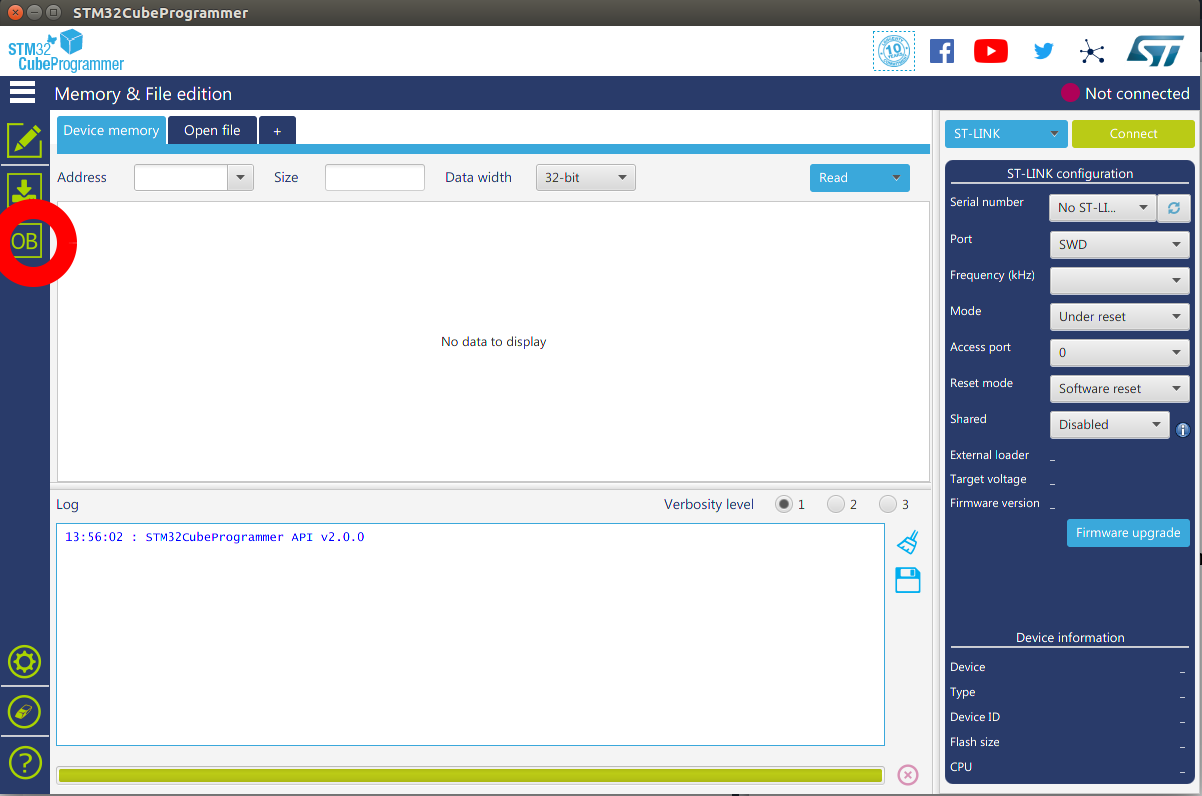
\includegraphics[keepaspectratio=true,scale=0.4]{stm32cubeprgm1.png}
\label{visina8}
\end{center}\end{figure}
Déchochez la case "RDP"
\begin{figure}[H]
\begin{center}
\advance\leftskip-3cm
\advance\rightskip-3cm
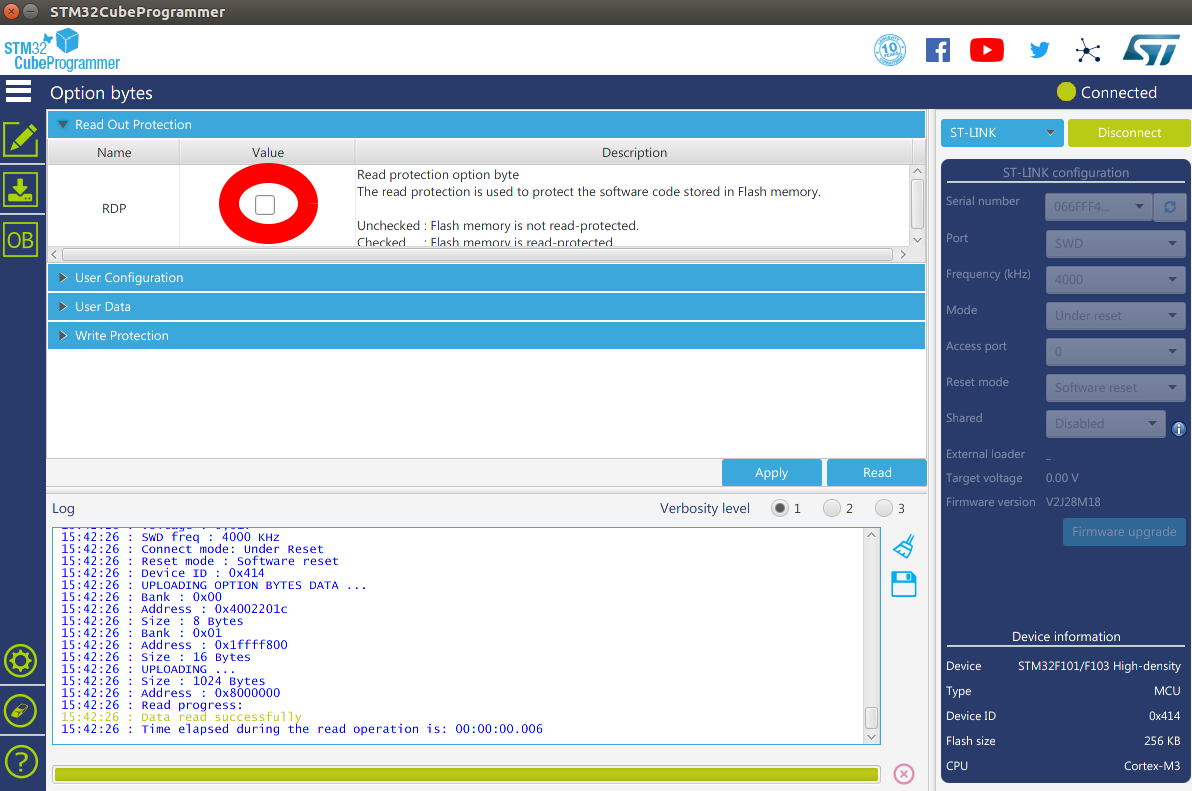
\includegraphics[keepaspectratio=true,scale=0.4]{stm32Cubeprogrammer_readoutprotection.png}
\label{visina8}
\end{center}\end{figure}

\section{Avec openOCD}
Ajoutez les 3 lignes suivantes dans RIOT/dist/tools/openocd/openocd.sh 

\begin{figure}[H]
\begin{center}
\advance\leftskip-3cm
\advance\rightskip-3cm
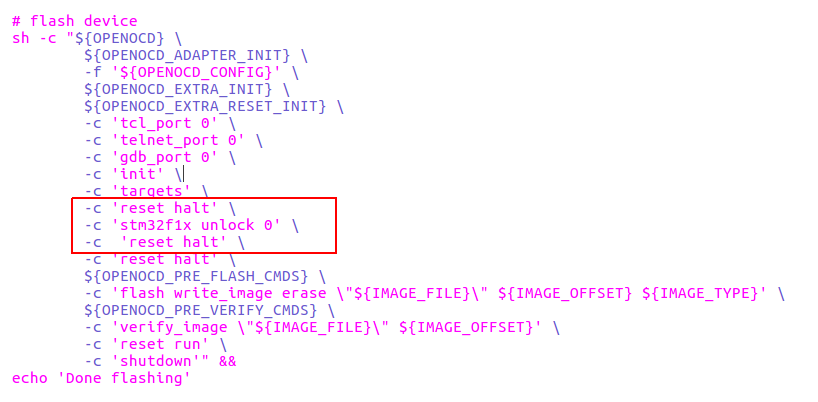
\includegraphics[keepaspectratio=true,scale=0.4]{openocddotsh.png}
\label{visina8}
\end{center}\end{figure}




\end{document}
